% context: 9th-grade physics unit test, Unit 2 kinematics with Unit 1 measurement
%        review; given 20 November 2026. Parallel to 2-8PreTest_Kinematics and
%        2-9HW_Kinematics-review, without mental math. Open notes: no formulas are
%        printed, only conversion factors, with distractors among them
% topic: significant figures, rounding, scientific notation with a calculator; a
%        one-chain unit conversion; a rate problem in two steps; distance vs
%        displacement, average speed vs velocity; constant acceleration from rest
%        (a jet's take-off run); a ball thrown up; reading a velocity-time graph;
%        reading labelled points on a height-time parabola; computing and plotting a
%        parabola and its velocity line
% structure: six pages; p1 conversions line, Q1-Q2; p2 Q3-Q4; p3 Q5-Q6; p4 the
%        velocity graph alone; p5 the labelled parabola (easier); p6 table and both
%        graphs to plot (harder). Mostly room to work
% skills (for competency scoring): Q1 sig figs, rounding, sci notation, calculator;
%        Q2 unit conversion; Q3 rate problem; Q4 displacement and average velocity;
%        Q5 constant-acceleration equations; Q6 free fall; Q7 motion graphs (v-t);
%        Q8 motion graphs (reading y-t); Q9 motion graphs (plotting y-t and v-t)
% design notes: one part per conversion; no back-references; no coincidental
%        values within a problem (checked); Q8 and Q9 use g = 10 m/s^2 so the points
%        land on grid lines, as in 2-7CW and 2-9HW Q7
% data: speed of light, Sun distance 1.496 x 10^8 km (contexts.md #10); cheetah
%        65 mi/h, 29 m/s measured (contexts.md #1); LaGuardia runways about 7000 ft.
%        The ride, the walk, the jet's acceleration, the throws and the car's graph
%        are chosen values
\documentclass[12pt, twoside]{article}
%\documentclass[12pt, twoside]{article}
\usepackage[letterpaper, margin=1in, headsep=0.2in]{geometry}
\setlength{\headheight}{0.6in}
%\usepackage[english]{babel}
\usepackage[utf8]{inputenc}
\usepackage{microtype}
\usepackage{amsmath}
\usepackage{amssymb}
%\usepackage{amsfonts}
\usepackage[nomessages]{fp} %\FPeval{\var-name}{2*sin(pi/6)}
\usepackage{siunitx} %units in math. eg 20\milli\meter
\usepackage{yhmath} % for arcs, overparenth command
\usepackage{tikz} %graphics
\usetikzlibrary{quotes, angles, arrows, arrows.meta}
\usepackage{graphicx} %consider setting \graphicspath{{images/}}
\usepackage{parskip} %no paragraph indent
\usepackage{enumitem}
\usepackage{multicol}
\usepackage{venndiagram}

\usepackage{fancyhdr}
\pagestyle{fancy}
\fancyhf{}
\renewcommand{\headrulewidth}{0pt} % disable the underline of the header
\raggedbottom
\hfuzz=2mm %suppresses overfull box warnings

\usepackage{hyperref}
\usepackage{float}

\title{Physics}
\author{Chris Huson}
\date{November 2026}

\fancyhead[LE]{\thepage}
\fancyhead[RO]{\thepage \\ Nickname: \hspace{2.25cm} \,\\ \,}
\fancyhead[LO]{La Scuola d'Italia / Huson / Physics \\* 20 November 2026}

\newcommand{\blank}[1][2.4cm]{\rule{#1}{0.4pt}}

\begin{document}

\subsubsection*{2.11 Test: Kinematics}

You may use your notes and a calculator. Show your work, with units, in the space
below each question.

\textbf{Conversions.} \quad
\mbox{1 min = 60 s} \quad \mbox{1 h = 60 min} \quad \mbox{1 h = 3600 s} \quad
\mbox{1 km = 1000 m} \\
\hspace*{2.65cm}\mbox{1 m/s = 3.6 km/h} \quad \mbox{1 mile = 1609 m} \quad
\mbox{1 ft = 0.3048 m}

\textbf{Free fall.} \quad $g = 9.80$ m/s$^2$ downward

\vspace{0.2cm}

\begin{enumerate}[itemsep=0.6cm]

\item Measurement review.
  \begin{enumerate}[itemsep=0.6cm]
    \item How many significant figures are in \num{0.06080} kg? \hfill \blank
    \item Round the speed of light, \num{299792458} m/s, to three significant
      figures. Write it in scientific notation. \hfill \blank
    \item The Sun is \num{149600000} km from Earth. Write this distance in meters,
      in scientific notation. \hfill \blank
    \item Light travels at $3.00 \times 10^{8}$ m/s. How many seconds does light
      from the Sun take to reach Earth?
      \vspace{3.2cm}
  \end{enumerate}

\item The fastest measured run by a cheetah was 65 mi/h. Convert this speed to m/s.
  Write the conversion as one chain of unit factors.

\newpage

\item A cyclist rides 12.5 km along the Hudson River Greenway at an average speed of
  4.6 m/s. How many minutes does the ride take?

  Step 1: find the time in seconds. \quad Step 2: convert it to minutes.
  \vspace{7.5cm}

\item Take the bus stop as the origin, with east positive. A student walks 9 m east
  in 6.0 s, then 25 m west in 14.0 s. Draw each displacement as an arrow above the
  number line.

  \begin{center}
  \begin{tikzpicture}[scale=0.5]
    \draw[<->, thick] (-17,0) -- (11,0) node[right]{$x$ (m)};
    \foreach \x in {-16,...,10} \draw (\x,0.12) -- (\x,-0.12);
    \foreach \x in {-16,-14,...,10} \node[below] at (\x,-0.12) {\small \x};
    \node[above] at (0,0.1) {\scriptsize bus stop};
    \path (0,0) -- (0,1.8); % room above the line for the arrows
    % Solution arrows — uncomment to see the answer
    %\draw[->, very thick] (0,0.8) -- (9,0.8) node[midway, above]{\small $+9$ m};
    %\draw[->, very thick] (9,1.6) -- (-16,1.6) node[midway, above]{\small $-25$ m};
  \end{tikzpicture}
  \end{center}

  \begin{enumerate}[itemsep=0.6cm]
    \item Where does the student end up? \hfill $x = $ \blank
    \item Distance walked = \blank \hfill Displacement = \blank
    \item Find the average speed and the average velocity for the whole walk.
  \end{enumerate}

\newpage

\item A passenger jet starts from rest at the end of the runway and speeds up at
  2.50 m/s$^2$. It lifts off the ground at 78.0 m/s.
  \begin{enumerate}[itemsep=0.4cm]
    \item How long does the jet take to reach lift-off speed?
      \vspace{2.4cm}
    \item How far along the runway does the jet travel before it lifts off?
      \vspace{3.0cm}
    \item The main runways at LaGuardia Airport are about 7000 ft (2130 m) long.
      Is that long enough for this jet? Explain.
      \vspace{0.6cm}
  \end{enumerate}

\item A tennis ball is thrown straight up at 14.7 m/s. Take \emph{up} as positive.
  \begin{enumerate}[itemsep=0.4cm]
    \item At the highest point, what is the ball's velocity? What is its
      acceleration?
      \vspace{0.8cm}
    \item How long does the ball take to reach the highest point?
      \vspace{1.9cm}
    \item How high does it go?
      \vspace{2.0cm}
    \item When does the ball come back to the thrower's hand, and what is its
      velocity then?
  \end{enumerate}

\newpage

\item The graph shows the velocity of a car between two traffic lights.

  \begin{center}
  \begin{tikzpicture}[x=0.82cm, y=0.36cm]
    \draw[gray!25, thin, xstep=0.5, ystep=1] (0,0) grid (16,16);
    \draw[gray!60, xstep=1, ystep=2] (0,0) grid (16,16);
    \draw[->, thick] (0,0) -- (16.5,0) node[right]{\small $t$ (s)};
    \draw[->, thick] (0,0) -- (0,17) node[above]{\small $v$ (m/s)};
    \foreach \t in {0,...,16} \node[below] at (\t,0) {\scriptsize \t};
    \foreach \v in {2,4,...,16} \node[left] at (0,\v) {\scriptsize \v};
    \draw[very thick] (0,0) -- (5,15) -- (9,15) -- (15,0);
  \end{tikzpicture}
  \end{center}

  \begin{enumerate}[itemsep=0.4cm]
    \item What is the car's velocity at $t = 2.0$ s? \hfill \blank
      \vspace{0.6cm}
    \item Find the car's acceleration from 0 to 5.0 s. Give the units.
      \vspace{2.6cm}
    \item What is the acceleration from 5.0 s to 9.0 s? What is the car doing?
      \vspace{1.8cm}
    \item Find the acceleration from 9.0 s to 15.0 s. What does its sign tell you?
      \vspace{2.6cm}
    \item Does the car ever move backward? How can you tell from the graph?
  \end{enumerate}

\newpage

\item A baseball is hit straight up at 30 m/s. Take \emph{up} as positive, and
  $g \approx 10$ m/s$^2$. The graph shows its height above the bat. The labelled
  points sit on grid lines.

  \begin{center}
  \begin{tikzpicture}[x=2.0cm, y=0.11cm]
    \draw[gray!25, thin, xstep=0.2, ystep=1] (0,0) grid (6.6,50);
    \draw[gray!60, xstep=1, ystep=5] (0,0) grid (6.6,50);
    \draw[->, thick] (0,0) -- (6.9,0) node[right]{\small $t$ (s)};
    \draw[->, thick] (0,0) -- (0,52.5) node[above]{\small $y$ (m)};
    \foreach \t in {0,...,6} \node[below] at (\t,0) {\scriptsize \t};
    \foreach \y in {10,20,...,50} \node[left] at (0,\y) {\scriptsize \y};
    \draw[very thick, domain=0:6, samples=80] plot (\x, {30*\x - 5*\x*\x});
    \foreach \t/\y/\n/\p in {0/0/A/above left, 1/25/B/above left, 3/45/C/above,
        5/25/D/above right, 6/0/E/above right}
      { \fill (\t,\y) circle (3pt); \node[\p] at (\t,\y) {\textbf{\n}}; }
  \end{tikzpicture}
  \end{center}

  \begin{enumerate}[itemsep=0.4cm]
    \item Read the time and height of each labelled point.

      {\renewcommand{\arraystretch}{1.5}%
      \begin{tabular}{| l | p{1.3cm} | p{1.3cm} | p{1.3cm} | p{1.3cm} | p{1.3cm} |}
        \hline
        Point & \centering A & \centering B & \centering C & \centering D &
          \centering\arraybackslash E \\ \hline
        $t$ (s) & & & & & \\ \hline
        $y$ (m) & & & & & \\ \hline
      \end{tabular}}
    \item Which point is the top? What are the ball's velocity and acceleration
      there?
      \vspace{0.7cm}
    \item Between which points is the ball going up? Coming down? How does the
      graph show it?
      \vspace{0.7cm}
    \item Draw the chord from A to C. Find its slope. What does it tell you?
      \vspace{1.3cm}
    \item The ball has the same height at B and at D. Find its velocity at B and
      at D. How are they alike, and how are they different?
      \vspace{1.3cm}
    \item What is the ball's velocity at E?
  \end{enumerate}

\newpage

\item A ball is tossed straight up from a student's hand at 8 m/s. Take \emph{up}
  as positive, with $y = 0$ at the hand, and $g \approx 10$ m/s$^2$.
  \begin{enumerate}[itemsep=0.4cm]
    \item Use your notes to show that the ball's height is $y = 8t - 5t^2$, and its
      velocity is $v = 8 - 10t$.
      \vspace{1.4cm}
    \item Fill in the table.

      {\renewcommand{\arraystretch}{1.5}%
      \begin{tabular}{| l | p{0.95cm} | p{0.95cm} | p{0.95cm} | p{0.95cm} |
          p{0.95cm} | p{0.95cm} | p{0.95cm} | p{0.95cm} | p{0.95cm} |}
        \hline
        $t$ (s) & \centering 0 & \centering 0.2 & \centering 0.4 & \centering 0.6 &
          \centering 0.8 & \centering 1.0 & \centering 1.2 & \centering 1.4 &
          \centering\arraybackslash 1.6 \\ \hline
        $y$ (m) & & & & & & & & & \\ \hline
        $v$ (m/s) & & & & & & & & & \\ \hline
      \end{tabular}}
    \item Plot $y$ against $t$ on the position grid, and join the points with a
      smooth curve. Plot $v$ against $t$ on the velocity grid, and join the points
      with a ruler.

      \begin{tikzpicture}[x=3.3cm, y=1.9cm]
        \draw[gray!25, thin, xstep=0.1, ystep=0.1] (0,0) grid (1.6,3.4);
        \draw[gray!60, xstep=0.2, ystep=0.5] (0,0) grid (1.6,3.4);
        \draw[->, thick] (0,0) -- (1.68,0) node[below right]{\small $t$ (s)};
        \draw[->, thick] (0,0) -- (0,3.6) node[above]{\small $y$ (m)};
        \foreach \t in {0,0.4,0.8,1.2,1.6} \node[below] at (\t,0) {\scriptsize \t};
        \foreach \y in {0.5,1.0,1.5,2.0,2.5,3.0} \node[left] at (0,\y) {\scriptsize \y};
        \node[above] at (0.8,3.6) {\small Position};
        % Solution curve — uncomment to see the answer
        %\draw[very thick, domain=0:1.6, samples=60] plot (\x, {8*\x - 5*\x*\x});
        %\foreach \t in {0,0.2,...,1.6} \fill (\t, {8*\t - 5*\t*\t}) circle (1.5pt);
      \end{tikzpicture}
      \hfill
      \begin{tikzpicture}[x=3.3cm, y=0.4cm]
        \draw[gray!25, thin, xstep=0.1, ystep=1] (0,-8) grid (1.6,8);
        \draw[gray!60, xstep=0.2, ystep=2] (0,-8) grid (1.6,8);
        \draw[->, thick] (0,0) -- (1.68,0) node[above right]{\small $t$ (s)};
        \draw[->, thick] (0,-8) -- (0,9) node[above]{\small $v$ (m/s)};
        \foreach \t in {0.4,0.8,1.2,1.6}
          \node[below, fill=white, inner sep=1pt] at (\t,-0.3) {\scriptsize \t};
        \foreach \v in {-8,-4,...,8} \node[left] at (0,\v) {\scriptsize \v};
        \node[above] at (0.8,9) {\small Velocity};
        % Solution line — uncomment to see the answer
        %\draw[very thick] (0,8) -- (1.6,-8);
        %\foreach \t in {0,0.2,...,1.6} \fill (\t, {8 - 10*\t}) circle (1.5pt);
      \end{tikzpicture}
    \item When is the ball highest, and how high does it go? What is its velocity
      at that moment?
      \vspace{1.0cm}
    \item Find the slope of the velocity graph, with units. What quantity is it?
  \end{enumerate}

\end{enumerate}
\end{document}
